
\subsection{Lepton+Jets}
The lepton$+$jets channel is the most statistically powerful decay of the $\ttbar$ system for measuring the pair-production cross-section.
The leptonic decay of one of the top results in an event topologiy that allows for strong background discrimination, while the hadronic decay of the other top maintains a high branching ratio for this channel.
The distinguishing features of the lepton$+$jets channel is the presence of a high-pt lepton from the leptonic decay of a W boson,v$\MET$ from a neutrino, two b-jets from the decay $t \rightarrow W+b$, and two additional jets from the hadronic decay of a W boson.
This topology of event was selected for by first requiring a single lepton trigger, which either required an electron or a muon (reconstructed by the trigger) with $E_{T} > 20 GeV$ or $p_{T} > 18 GeV$, respectively.
The exact trigger required varied throught the run periods of 2011 as higher instintaneous luminosities required stricter lepton definitions to maintain a steady bandwidth of recorded events as selected by the trigger.
Selected events are required to have a primary vertex that consists of 5 or more tracks.
Each event must have exactly 1 selected electron or muon, and that lepton must match a corresponding object that fired a single-lepton trigger (events with more than 1 lepton fall into the dilepton channel, to be described in detail later).
The energy requirements for these objects were chosen to minimize any effects resulting from the trigger's online reconstruction.
A cut on $\MET$ is imposed, requiring $\MET > 35 GeV$ for the electron channel and $\MET > 25 GeV$ for the muon channel (the difference in the cut results from different background contributions to each channel from QCD events, which tend to have low values of $\MET$).
Additional cuts are made on the to reduce the contamination from QCD, which use a variable known as the ``W boson transverse mass'':
\begin{equation}
  m_{T}(W) = \sqrt(2 p_{T}^{l} p_{T}^{\nu} (1 - cos( \phi^{l} - \phi^{\nu}))),
\end{equation} 
where the $\MET$ vector is used to determine the kinematic variables of the neutrino, $p_{T}^{\nu}$ and $\phi^{\nu}$.
Using this definition, the event selection requires $m_{T}(W) > 25 GeV$ in the electron channel or $\MET + m_{T}(W) > 60 GeV$ in the muon channel.



\subsubsection{Backgrounds}
A selection of events based on the above criteria will be contaminated with several sources of backgrounds, including

\begin{itemize}
\item QCD Multijet events where a lepton is faked via a background mechanism
\item $W+Jets$ events where the W decays leptonically (leading to $\MET$) which includes real or fake b-jets
\item $Z+Jets$ events where one of the two leptons isn't identified and which includes real or fake b-jets
\item Diboson Events (WW, WZ, or ZZ events), that include some combination of leptonic decays of vector bosons, additional jets, and real or faked b-jets
\item Single Top events
\end{itemize}

% Add figures

\begin{figure}
  \begin{center}
    \subfigure[$W+Jets$]{
      % 
      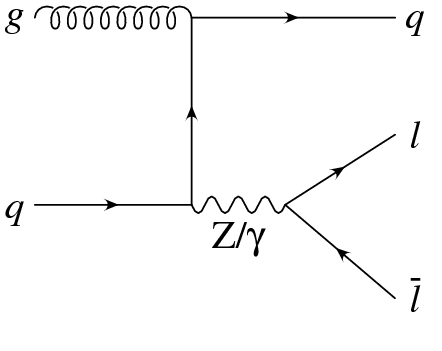
\includegraphics[width=.4\linewidth]{figures/xsection/ZJetsDiagram.png}
    }
    \subfigure[$QCD$]{
      %ZJetsDiagram.png : http://inspirehep.net/record/871058/files/qg_qZ.png
      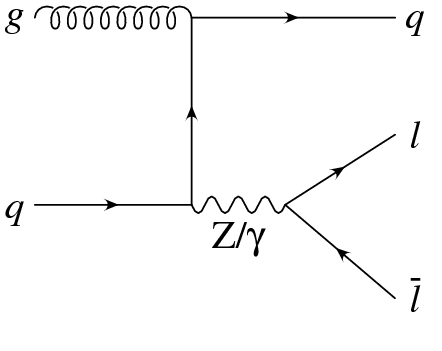
\includegraphics[width=.4\linewidth]{figures/xsection/ZJetsDiagram.png}
    } \\
    \subfigure[$Z+Jets$]{
      %ZJetsDiagram.png : http://inspirehep.net/record/871058/files/qg_qZ.png
      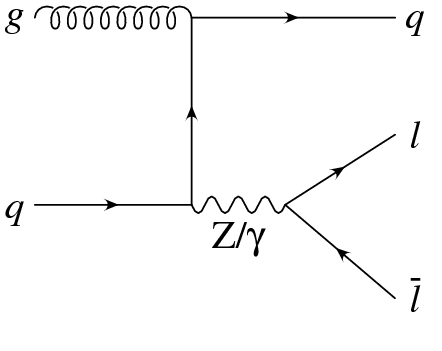
\includegraphics[width=.4\linewidth]{figures/xsection/ZJetsDiagram.png}
    }
    \subfigure[$Single Top$]{
      % 
      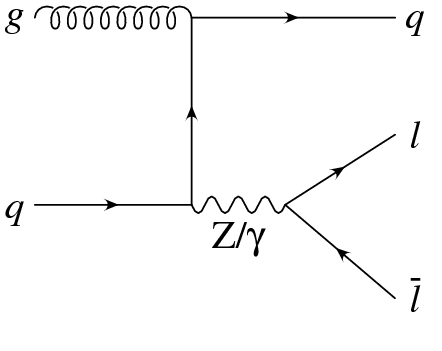
\includegraphics[width=.4\linewidth]{figures/xsection/ZJetsDiagram.png}
    } \\
  \end{center}
  \caption{Feynman diagrams for the most important backgrounds to $\ttbar$ events.  Shown are $Z+Jets$ events (top, left), $W+jets$ events (top, right), QCD events (bottom, left) and Single Top events (bottom, right).}
  \label{img:BackgroundsFeynmanDiagrams}
\end{figure}

To measure the cross-section, the background contributions due to each of the above processes in the lepton+jets channel were determined using a variety of techniques.
The dominant $W+Jets$ background as well as the $Z+Jets$, diboson, and single-top background are estimated using Monte-Carlo simulation.
While the kinematic distributions of each $W+Jets$ event were estimated from Monte-Carlo, the expected number of events was extracted using a data-driven technique.
The technique used to estimate the normalization of the $W+Jets$ background is based on one used in a top-quark charge-asymmetry analysis \cite{CHARGE_ASYMMETRY}.
It is based on the fact that $W^{+}$ bosons are produced at a higher rate than $W^{-}$ bosons due to the fact that the LHC collides protons (and not anti-protons).
The ratio of the production of $W^{+}$ to $W^{-}$, $r_{MC}$, can be estimated using Monte-Carlo.  Assuming that $W+Jets$ events are the dominant category of events that are asymmetric between positive and negative leptons, one can estimate the total number of $W+Jets$ events by taking the difference between the measured jumber of events with a positive lepton and the number with a negative lepton:

\begin{equation}
  N_{W^{+}} + N_{W^{-}} = \frac{r_{MC} + 1}{r_{MC} - 1}(D^{+} - D^{-}),
\end{equation}

where $D^{+}$ and $D^{-}$ are the number of selected single-lepton events with a positive or negative lepton, respectively.
The value of $r_{MC}$ is measured to be 1.56 $\pm$ 0.07 for the electron channel and 1.66 $\pm$ 0.06 for the muon channel.
Estimates of overall yields or kinematic variables for the $W+Jets$ background are then weighted to a total normalization given by this data-driven value.
The normalizations for the $Z+Jets$, diboson, and single-top backgrounds are taken directly from cross-sections evaluated using monte-carlo and scaled to the integrated luminosity recorded by the ATLAS detector.

Each of the backgrounds which are estimated using Monte-Carlo lead to real leptons in the final state.
In contrast, the QCD background enters the single-lepton channel when a final state jet is falsely identified as a lepton.
The process of a jet faking a lepton depends on the details of the jet's hadronic shower, in particular it's shape and depth in both the electromagnetic and hadronic calorimeters.
The hadronic shower evolution is of course modeled in detail by simulations used by ATLAS.
However, small differences in the nature of that simulation can lead to significant changes in the rate of jets faking leptons.
And because the number of QCD events created at ATLAS is extremely large, changes in the rate will have dramatic differences in the number of background events in the lepton+jets signal region.
For this reason, it is preferable to estimate the background contribution due to QCD without relying on the details of the Monte-Carlo description of hadronic shower evolution.

The lepton+jets analysis uses a technique to extract the rate and distribution of QCD events from data directly.
Known as the ``Matrix Method,'' this technique exploits the fact that the efficiencies of real and fake leptons differ as a function of cuts on the reconstructed lepton's isolation and shower shape.
The technique involves creating two subsets of lepton identifications, denoted as ``loose'' and ``tight'' (with ``tight'' corresponding to the nominal selection requirements).
The Matrix Method relies on knowing the effecienciy for both real and fake leptons which pass loose selection to also pass the tight selection.

\begin{equation}
  \epsilon_{real} = \frac{N^{tight}_{real}}{N^{loose}_{real}} and \epsilon_{fake} = \frac{N^{tight}_{fake}}{N^{loose}_{fake}},
\end{equation}

where $N^{tight}$ and $N^{loose}$ represent the number of events with tight or loose (and not tight) lepton, respectively, in the region of phase space where the efficiency is being measured.
Given these values, one can write a set of equations relating the number of events with a measured loose or tight lepton to the number  

\begin{eqnarray}
  \bar{N^{tight}} = \epsilon_{real} N_{real} + \epsilon_{fake} N_{fake} \\
  \bar{N^{loose}} = (1-\epsilon_{real}) N_{real} + (1-\epsilon_{fake}) N_{fake}.
  \label{eq:MatrixMethod}
\end{eqnarray}

The above equations can be inverted to obtain $N_{fake}$ and $N_{real}$, quantities we're interested in estimating, as a function of  $N^{tight}$ and $N^{loose}$, quantities that can be measured.
By solving and isolating the variables $N^{tight}_{real}$ and $N^{tight}_{fake}$ (which represent the real and fake lepton contributions to the tight, or signal, region), and expressing the solution as a matrix, we obtain the following:

\begin{eqnarray}
  N^{tight}_{real} = \frac{N^{tight} - \epsilon_{fake}N^{loose}}{\epsilon_{fake} - \epsilon_{real}} \\
  N^{tight}_{fake} = \frac{\epsilon_{real}N^{loose} - N^{tight}}{\epsilon_{fake} - \epsilon_{real}}
\end{eqnarray}

\begin{equation}
\begin{pmatrix} N^{tight}_{real} \\ N^{tight}_{fake} \\ \end{pmatrix} 
  = 
  \begin{pmatrix} 
    \frac{\epsilon_{real}}{\epsilon_{real} - \epsilon_{fake}} & \frac{-\epsilon_{real}\epsilon_{fake}}{\epsilon_{real} - \epsilon_{fake}} \\ 
    \frac{-\epsilon_{fake}}{\epsilon_{real} - \epsilon_{fake}} & \frac{\epsilon_{real}\epsilon_{fake}}{\epsilon_{real} - \epsilon_{fake}} \\ 
  \end{pmatrix}  
  \begin{pmatrix} N^{tight} \\ N^{loose} \\ \end{pmatrix}
  \label{eq:MatrixMethodInverted}
\end{equation}

One should note that the solution is linear in the number of tight or loose events.
In particular, this means that we can associate any given event (be it loose or tight) with a weight for real or fake, and these weights are simply the (1,1) and (2,1) elements of the matrix in equation \ref{eq:MatrixMethodInverted}.
Therefore, in the case that the $\epsilon$ values are functions of arbitrary variables associated with an event, one can still estimate the number of fakes in the tight (signal) region as:

\begin{equation}
  N^{tight}_{fake} = \sum_{e \in tight} (\frac{-\epsilon_{fake}}{\epsilon_{real} - \epsilon_{fake}}) + \sum_{e \in loose} (\frac{\epsilon_{real}\epsilon_{fake}}{\epsilon_{real} - \epsilon_{fake}})
  \label{eq:MatrixMethodSum}
\end{equation}

Equation \ref{eq:MatrixMethodSum} is used to estimate the amount of QCD multijet events that enter the signal region (assuming that all fakes in the loose or tight regions come from QCD Multijet events).
In that estimation, loose electrons are defined identically as tight electrons, except their isolation cut is relaxed, requiring that $E_{T} < 6 GeV$ in a cone defined by $\Delta R = 0.2$.
Similarly, loose muons are identical to tight muons, but the cuts on $E_{T}$ and $p_{T}$ isolation are removed entirely.
The efficiencies for loose leptons, as defined above, to also pass tight requirements for both real and fake muons are measured directly in data.
To measure the efficiencies of real leptons, a collection of events dominated by $Z->ee$ or $Z->\mu\mu$ is created by selecting dilepton events where the invariant mass of the leptons is close to the mass of the Z-boson.
In such a sample, the efficiency can be measured directly.
For fake leptons, a sample of QCD multijet events is collected by selecting events with a single (loose) lepton, a jet, and by requiring $5 GeV < \MET <  60 GeV$ for electron events or $m_{T}(W) < 20 GeV$ and $m_{T}(W) + \MET < 60 GeV$ for muon events.
For muons, the efficiencies were paramaterized as a function of the muon's $p_{T}$ and $\eta$.
Contributions from $Z+Jets$ and $W+Jets$ in the QCD control regions were subtracted using Monte-Carlo estimates.

% e + Jets
\begin{table}
  \begin{tabular}{lccccc}
    \hline
    $e + Jets$ & 1 Jet & 2 Jet & 3 Jet & 4 Jet & $>=$ 5 Jets \\ 
    \hline
    $\ttbar$ & $225 \pm 15$ & $1005 \pm 32$ & $1934 \pm 44$ & $1835 \pm 43$ & $1463 \pm 38$ \\
    $W+Jets$ & $161600 \pm 400$ & $43170 \pm 210$ & $10840 \pm 100$ & $2486 \pm 50$ & $1032 \pm 32$ \\
    $QCD Multijets$ & $11000 \pm 5000$ & $4800 \pm 2400$ & $1600 \pm 800$ & $510 \pm 250$ & $117 \pm 89$ \\
    Single Top & $571 \pm 24$ & $711 \pm 27$ & $391 \pm 20$ & $156 \pm 13$ & $65 \pm 8$ \\
    $ZJets$ & $3732 \pm 61$ & $2444 \pm 49$ & $996 \pm 32$ & $333 \pm 18$ & $146 \pm 12$ \\
    Diboson & $599 \pm 25$ & $538 \pm 23$ & $178 \pm 13$ & $45 \pm 7$ & $10 \pm 3$ \\
    \hline
    Total Predicted & $177000 \pm 5000$ & $52600 \pm 2400$ & $15900 \pm 800$ & $5360 \pm 260$ & $2892 \pm 100$ \\
    Total Observed & 179469 & 51820 & 15614 & 5398 & 2812 \\
    \hline
  \end{tabular}
  \caption{Predicted and observed event yields in bins of jet number for the $\ttbar$ signal and backgrounds in the $e+jets$ channel.  Yields are obtained using Monte Carlo or Data-Driven techniques, depending on the sample.}
\end{table}

% mu + Jets
\begin{table}
  \begin{tabular}{lccccc}
    \hline
    $e + Jets$ & 1 Jet & 2 Jet & 3 Jet & 4 Jet & $>=$ 5 Jets \\ 
    \hline
    $\ttbar$ & $319 \pm 18$ & $1342 \pm 37$ & $2734 \pm 52$ & $2714 \pm 52$ & $2030 \pm 45$ \\
    $W+Jets$ & $383200 \pm 600$ & $93440 \pm 310$ & $20140 \pm 140$ & $4644 \pm 68$ & $1082 \pm 33$ \\
    $QCD Multijets$ & $25000 \pm 12000$ & $11000 \pm 6000$ & $3200 \pm 1600$ & $900 \pm 400$ & $290 \pm 150$ \\
    Single Top & $996 \pm 32$ & $1148 \pm 34$ & $594 \pm 24$ & $210 \pm 15$ & $84 \pm 9$ \\
    $ZJets$ & $17270 \pm 130$ & $5492 \pm 74$ & $1510 \pm 39$ & $436 \pm 21$ & $149 \pm 12$ \\
    Diboson & $1093 \pm 33$ & $1009 \pm 32$ & $308 \pm 18$ & $69 \pm 8$ & $18 \pm 4$ \\
    \hline
    Total Predicted & $428000 \pm 12000$ & $113000 \pm 6000$ & $28400 \pm 1600$ & $8900 \pm 400$ & $3660 \pm 160$ \\
    Total Observed & 433931 & 111741 & 28643 & 8680 & 3814 \\
    \hline
  \end{tabular}
  \caption{Predicted and observed event yields in bins of jet number for the $\ttbar$ signal and backgrounds in the $\mu+jets$ channel.  Yields are obtained using Monte Carlo or Data-Driven techniques, depending on the sample.}
\end{table}


\begin{figure}
  \begin{center}
    \subfigure[$e+jets$] {
      % EJetsYieldPlot.eps: https://atlas.web.cern.ch/Atlas/GROUPS/PHYSICS/CONFNOTES/ATLAS-CONF-2011-121/fig_01a.eps
      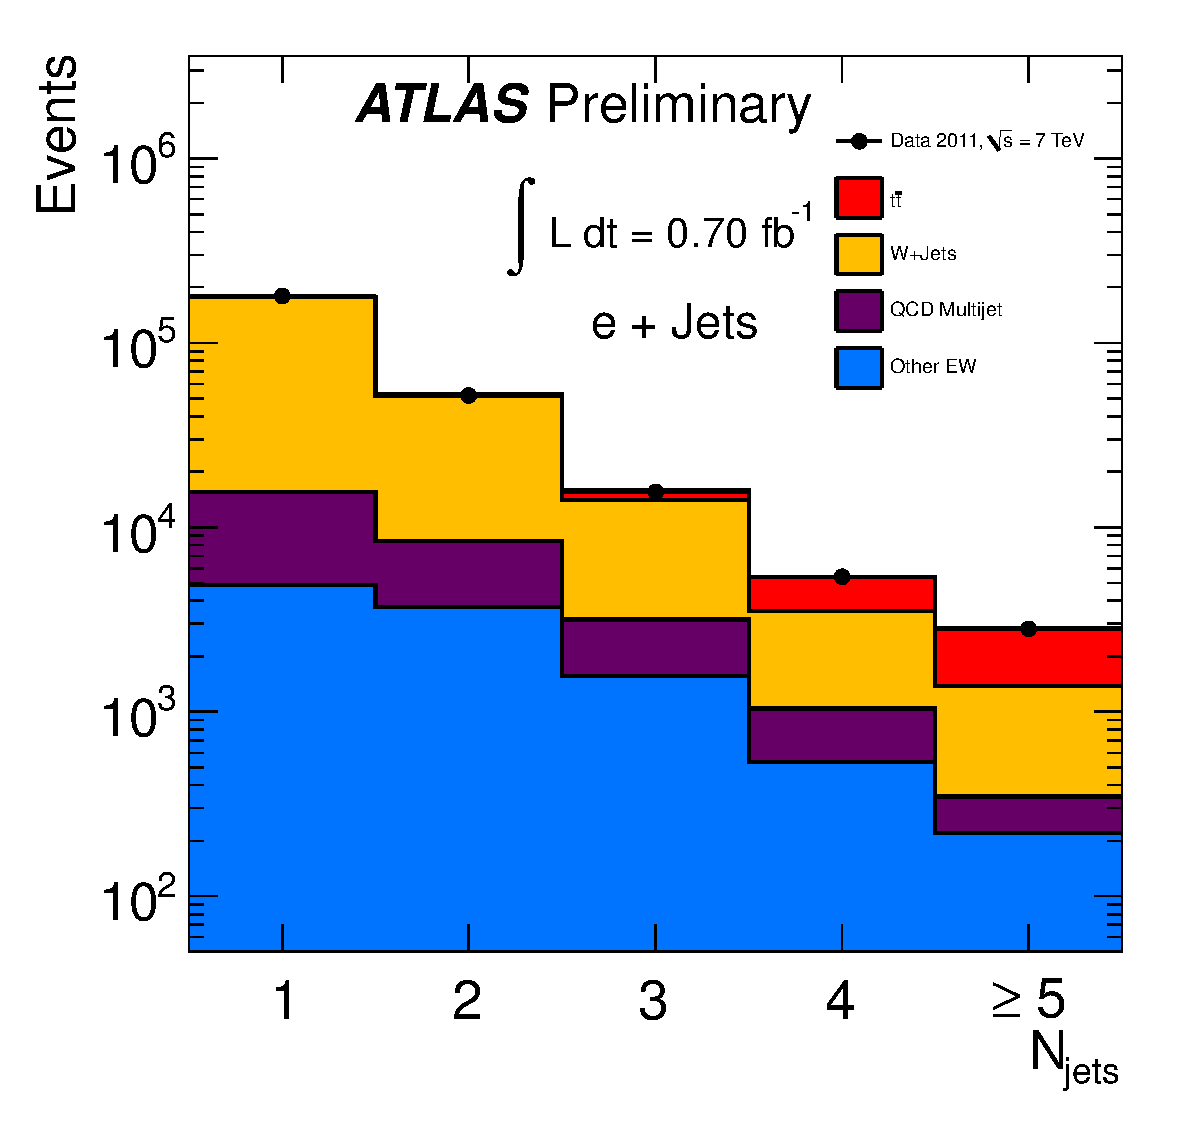
\includegraphics[width=.45\linewidth]{figures/xsection/EJetsYieldPlot}
    }
    \subfigure[$\mu+Jets$] {
      % MuJetsYieldPlots.eps: https://atlas.web.cern.ch/Atlas/GROUPS/PHYSICS/CONFNOTES/ATLAS-CONF-2011-121/fig_01b.eps
      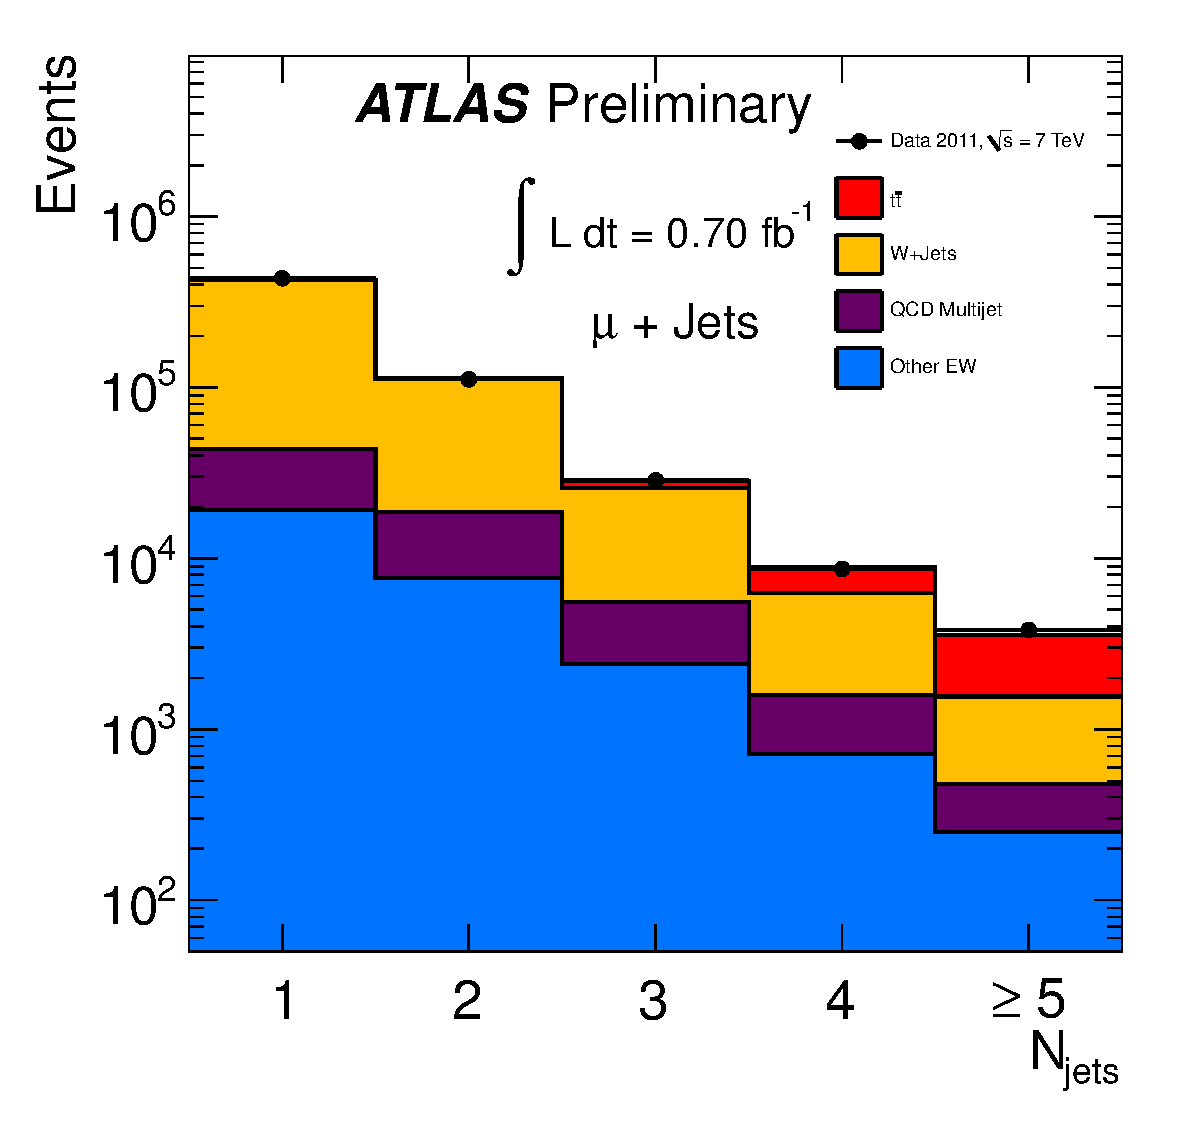
\includegraphics[width=.45\linewidth]{figures/xsection/MuJetsYieldPlot} %  figures/xsection/MuJetsYieldPlots}
    }
  \end{center}
  \caption{The yields of signal and backgrounds in bins of jet number.}
  \label{img:JetNumberYieldPlots}
\end{figure}


% https://atlas.web.cern.ch/Atlas/GROUPS/PHYSICS/CONFNOTES/ATLAS-CONF-2011-121/fig_01a.eps
% https://atlas.web.cern.ch/Atlas/GROUPS/PHYSICS/CONFNOTES/ATLAS-CONF-2011-121/fig_01b.eps


The measurement of the $\ttbar$ cross-section is obtained by fitting multiple multivariate distributions to measured data simultaneously.
These distributions are built out of four kinematic variables: the pseudorapidity of the selected lepton, the $p_{T}$ of the jet with the highest $p_{T}$, the event aplanrity and a variable denoted as $H_{T,3p}$.
The aplanarity, $A$, is defined as 1.5 times the smallest eivenvalue of the matrix

\begin{equation}
  M_{i,j} = \frac{ \sum_{k=1}^{N'_{objects}} p_{ik}p_{jk} }{ \sum_{k=1}^{N'_{objects}} p_{k}^2 }
  \label{eq:Aplanarity}
\end{equation}

and $H_{T, 3p}$, which is the total transverse momentum of all jets except for the first two normalized to the longitudinal momenta of all objects, is given by:

\begin{equation}
  H_{T, 3p} = \frac{ \sum_{i=3}^{N_{jets}} |p_{T, i}| }{ \sum_{j=1}^{N_{objects}} |p_{Z,j}|  }
\end{equation}


\begin{figure}
  \begin{center}
    \subfigure[leading jet $p_{T}$] {
      % DiscrimPtjet4Jets: https://atlas.web.cern.ch/Atlas/GROUPS/PHYSICS/CONFNOTES/ATLAS-CONF-2011-121/fig_04c.eps
      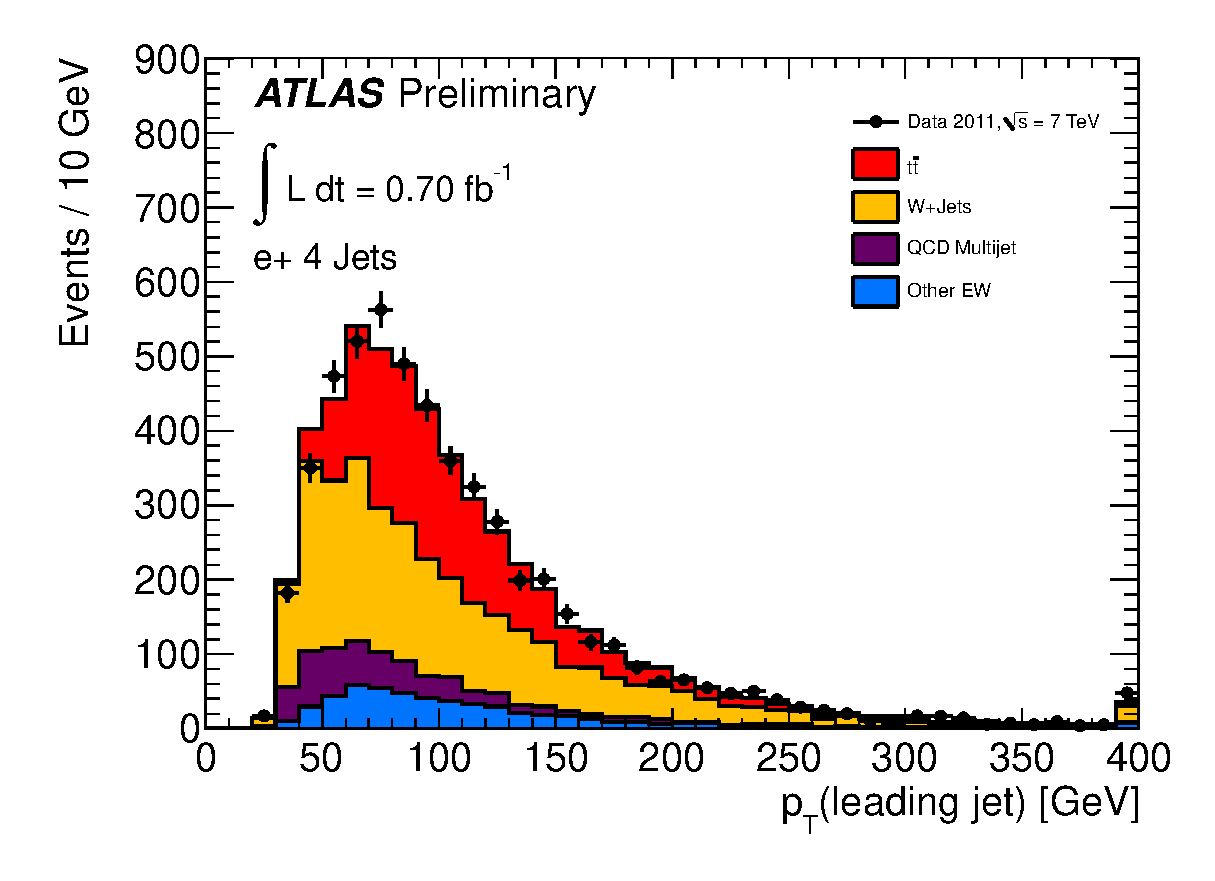
\includegraphics[width=.45\linewidth]{figures/xsection/DiscrimPtjet4Jets}
    }
    \subfigure[lepton ${\eta}$] {
      % DiscrimEtaMu4Jets
      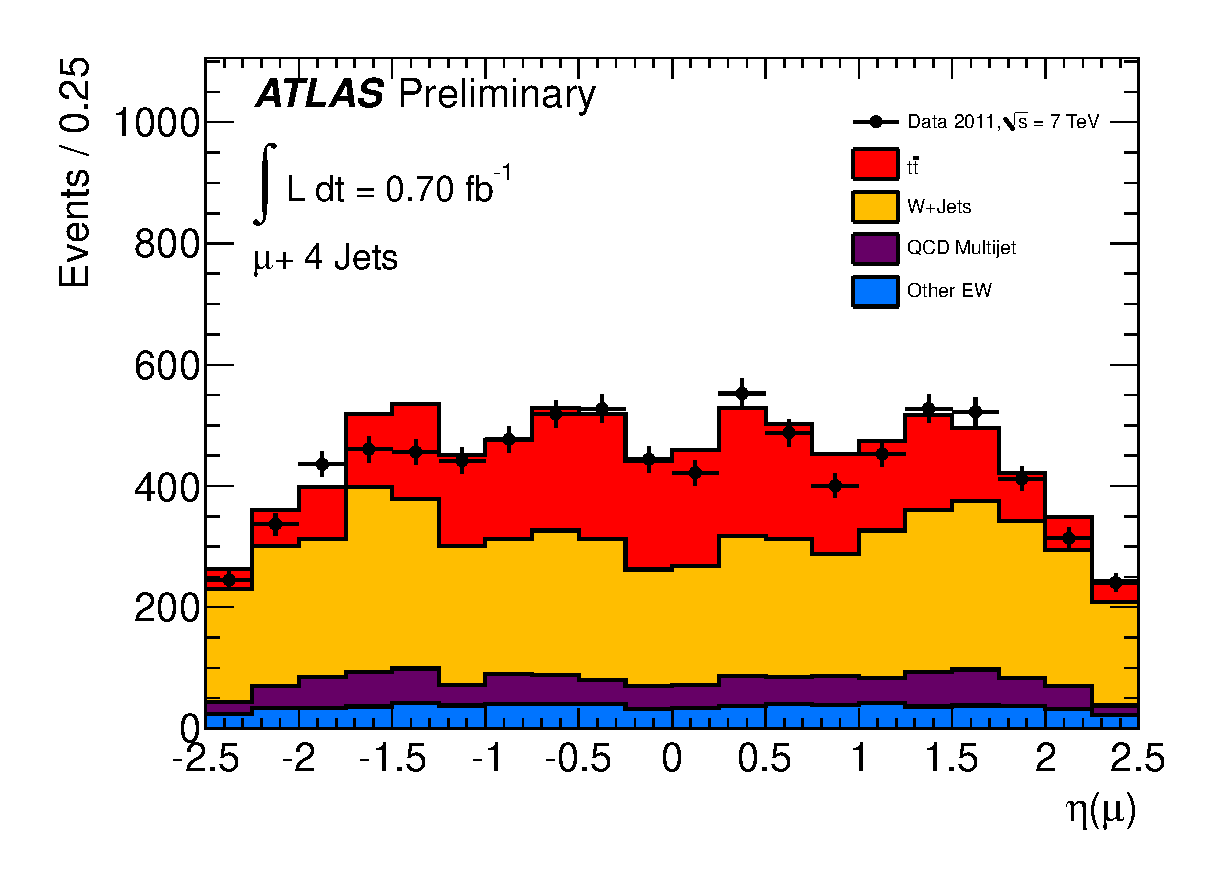
\includegraphics[width=.45\linewidth]{figures/xsection/DiscrimEtaMu4Jets}
    } 
    \subfigure[Aplanarity] {
      % 
      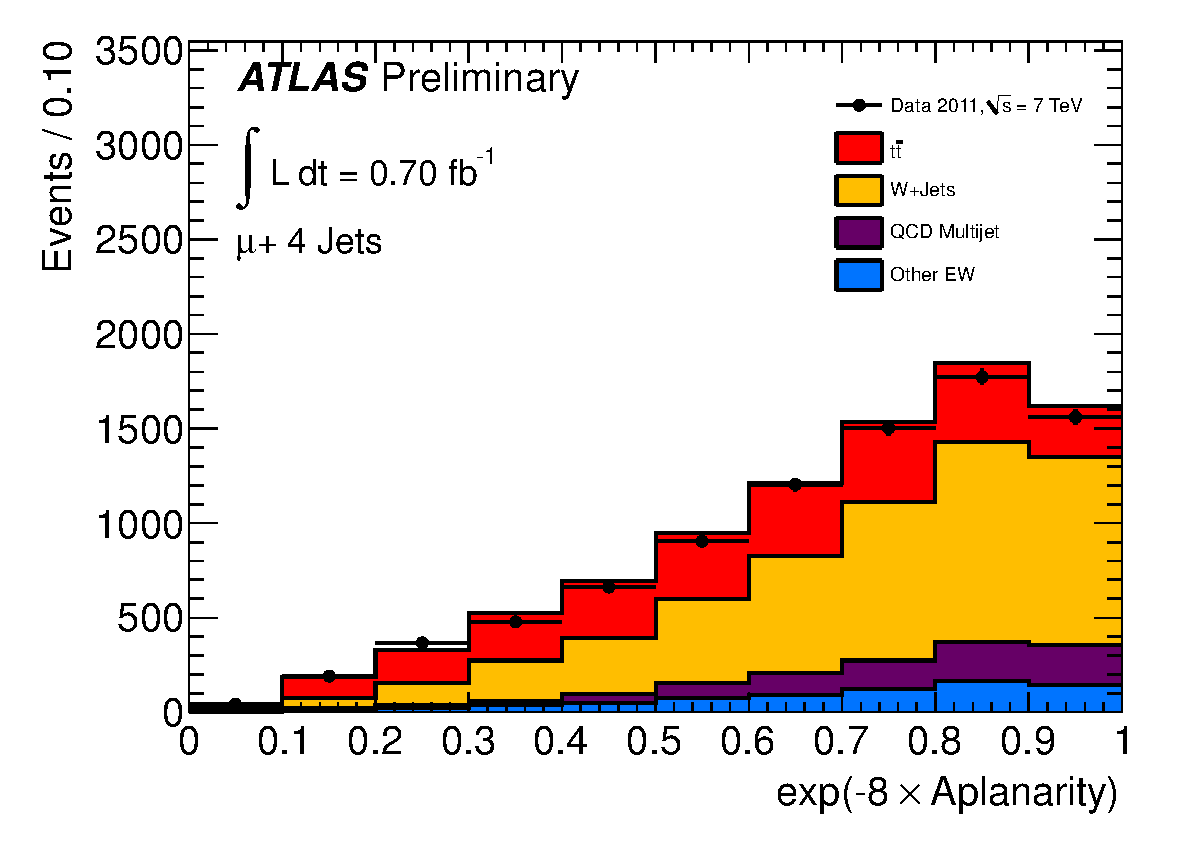
\includegraphics[width=.45\linewidth]{figures/xsection/DiscrimAplanarity4Jets}
    }
    \subfigure[$H_{T,3p}$] {
      % 
      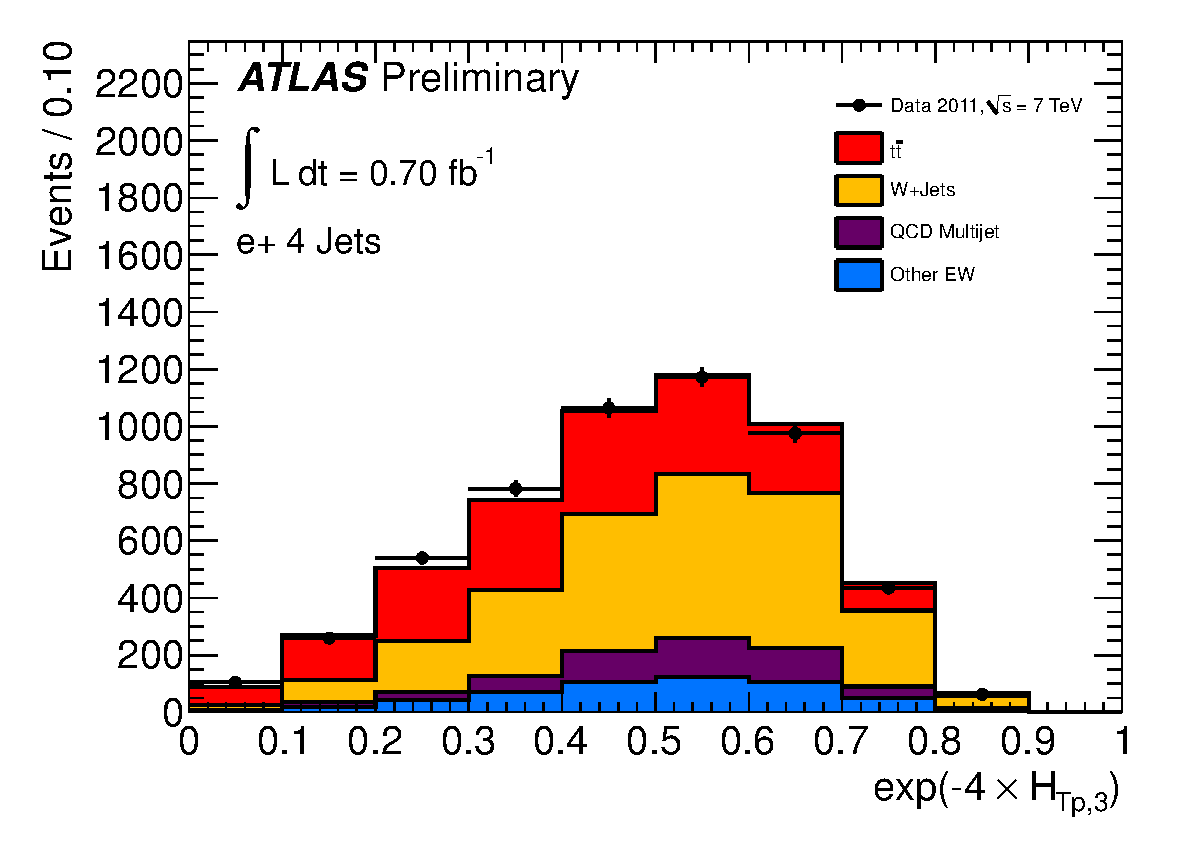
\includegraphics[width=.45\linewidth]{figures/xsection/DiscrimHT34Jets}
    } 
  \end{center}
  \caption{The discriminating variables used in the multivariate likelihood.}
  \label{img:DiscriminatingVariables}
\end{figure}


\begin{figure}
  \begin{center}

    \subfigure[] {
      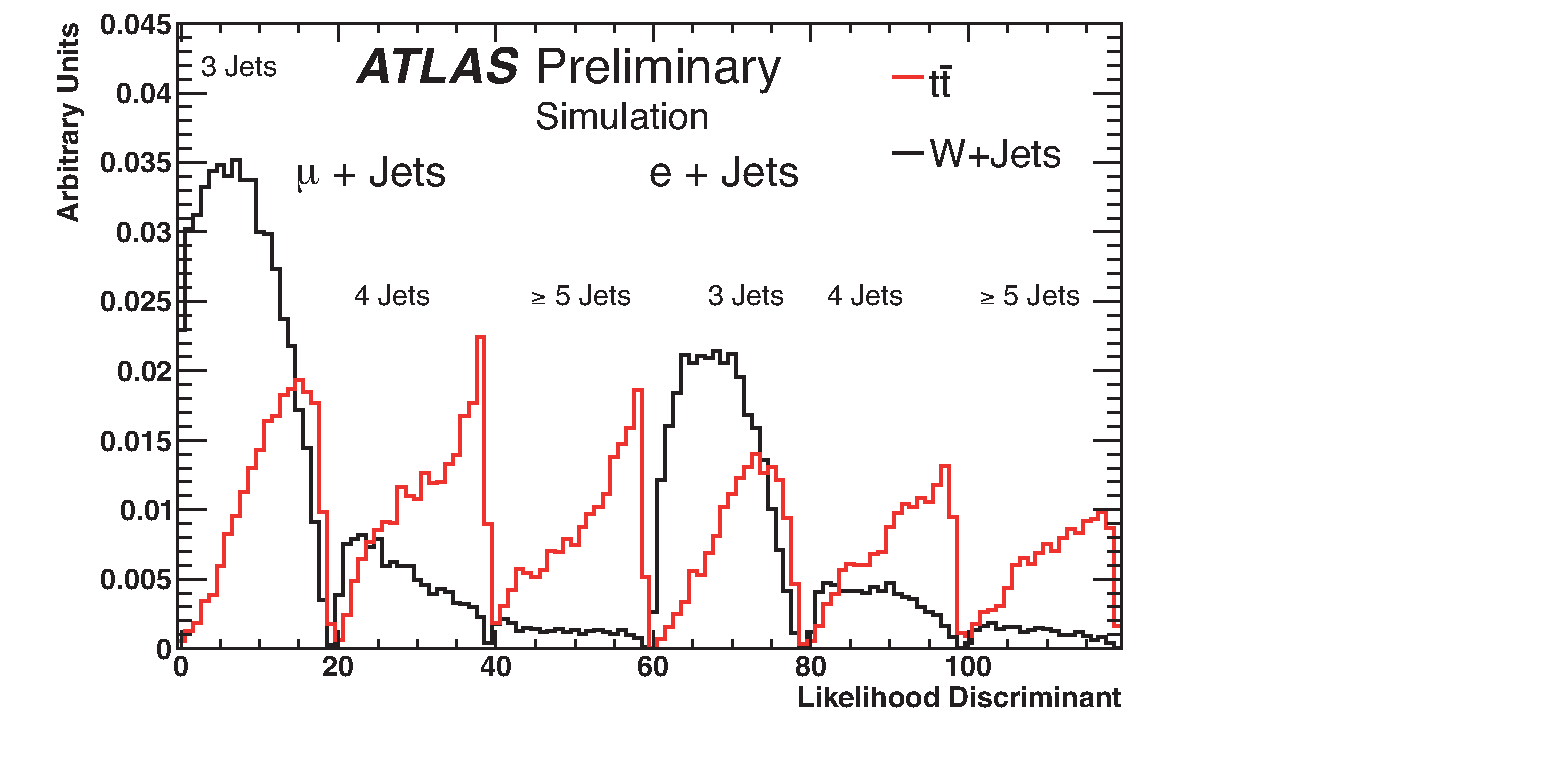
\includegraphics[width=.95\linewidth]{figures/xsection/LJetsDiscriminantLikelihood}
    }
    \subfigure[] {
      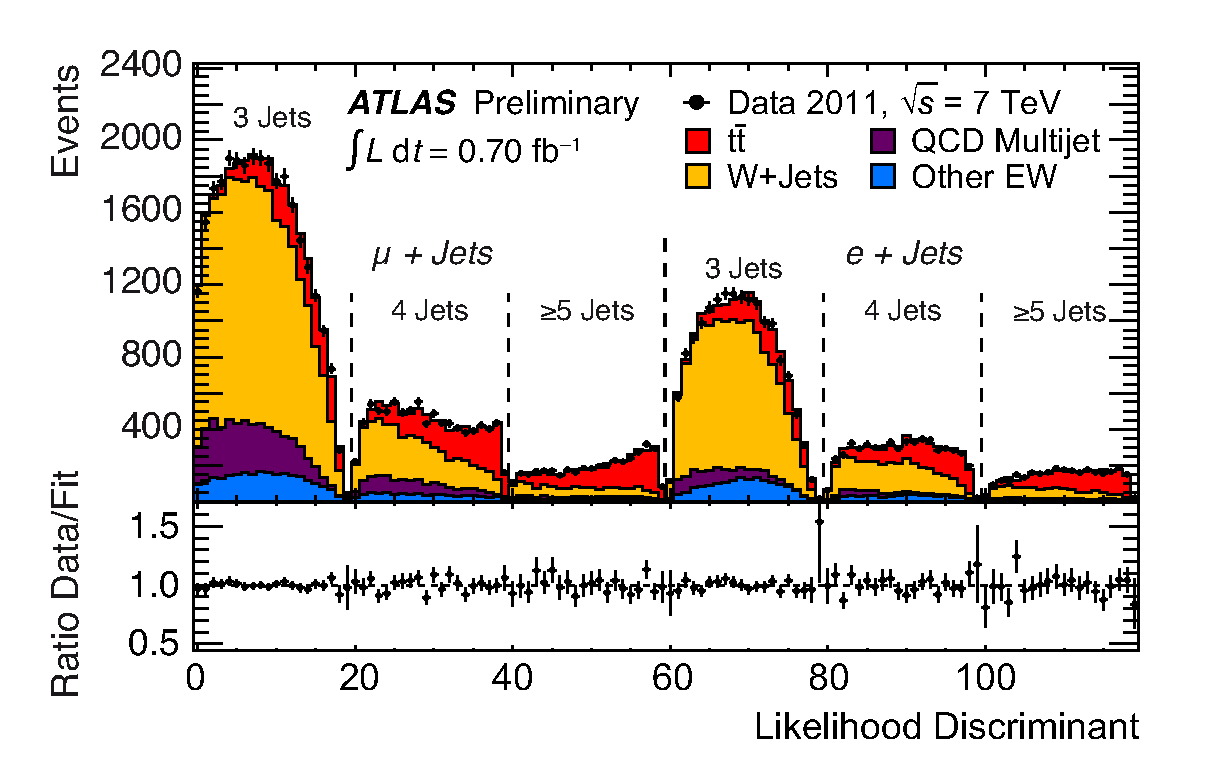
\includegraphics[width=.95\linewidth]{figures/xsection/LJetsFittedLikelihoodDiscriminant}
    }
  \end{center}
  \caption{The multivariate discriminant for $\ttbar$ signal and the dominant $W+Jets$ background.  Distributions are normalized to emphacize the difference in shape between signal and background.}
  \label{img:LJetsLikelihoodDiscriminant}
\end{figure}


\subsection{Systematic Uncertainties}

% The careful and consistent of the effect of systematic uncertainties and their proper paramaterization in a likelihood are crucial to making precise measurements.
The expected distribution of the discriminating variable in each channel and both signal and each background are sensitive to differences in theortical predictions and modeling of experimental effects.
Differences in the expected distributions will lead to differences in the measured cross-section.
Therefore, to incorporate theoretical and experimental uncertainties that will effect the measured cross-section, the expected distributions of the discriminating variable (including their normalizations as a function of integrated luminosity) are paramaterized by a number of terms that each represent on source of systematic uncertainty.
The likelihood function includes the effect of these parameters on the expected distributions as well as terms constraining these parameters, where the level of constraint comes from additional measurements that are made to gauge the size of these systematic uncertainties.
In the lepton+jets analysis, these constraints are modeled as gaussian terms with a mean of 0.0 and a variance of 1.0 (or rather, each paramater is scaled such that its constraint terms can be modeled in this way).

In the lepton+jets analysis, these uncertainties fall into several categories.  
Uncertainties on the cross-sections of backgrounds estimated using monte-carlo lead directly to uncertainties on the number of expected events in each bin of the discriminating variable for a fixed integrated luminosity.
These uncertainties on the cross-sections of the diboson, single-top and Z$+$Jet processes are determined by theoretical studies using Monte-Carlo simulation.
Uncertainties on the normalizations of the data-driven W$+$Jets and QCD backgrounds come from the propogation of statistical uncertainties through the data-driven techniques.
These data-driven normalization uncertainties are considered to be uncorrelated across in the 3 Jets, 4 Jets, and 5+ Jets channels (meaning, the effect is modeled by a separate parameter for each channel, and these parameters each have separate constraint terms and are allowed to move independently in a fit).

Uncertainties on the identification, reconstruction, and measurement of physical objects (jets, leptons, and $\MET$) effect the number of events that are selected, which channels those events may fall into, and the shape of discriminating variables within that channel.
These uncertainties include the energies of reconstructed objects as well as the rate at which they are triggered and identified.
Uncertainties on the measured energies of particles include uncertainties on both the energy scale and the energy resolution (roughly, these correspond to the mean and width of the distribution of measured energy, respectively).
The size of the uncertainties on object energy scale and energy resolution are paramaterized by many parameters of the object, but most importantly its position in the detector (in $\eta$ and $\phi$) and its nominal measured energy. [**]
The effect of energy uncertainties are estimated by rescaling or randomly smearing the energy of objects in Monte-Carlo and obtaining new histograms of the discriminating variables for each background and sample.
Two such sets of template histograms are created for each source of systematic uncertainty corresponding to the effect of a +1 sigma and -1 sigma shift in these parameters (in addition to the nominal histograms, which in this language correspond to a 0 sigma shift in all systematic uncertainties).
The shapes of discriminating histograms for arbitrary shifts in uncertainty parameters are obtained by interpolating between these templates.
Furthermore, uncertainties in the Jet Energy Scale are broken down into subcomponents which consider separately uncertainties on the JES due to the calorimeter, uncertainties due to extrapolating from a low b-jet region to a high b-jet region, the dependence of calibration on pseudorapidity, the modeling of jets across generators, the effect of pile-up, and the effect of the underlying event.

Similarly, uncertainties on the rate at which leptons are identified and triggered are paramaterized by the object's location and energy.[**]
The effect of these uncertainties on the expected distribution of signal and background events estimated from Monte-Carlo are estimatied by scaling the weight of individual events by a factor corresponding to the estimated difference between trigger, reconstruction, and identification rates between Monte-Carlo and data.
These scale factors are derived by studying known processes in data and comparing these processes to Monte Carlo (for leptons, these measurements are performed using Z boson events, where one can create a set of events with a high rate of real to fake leptons).

In addition, uncertainties on the modeling of initial and final state radiation (isr and fsr) in Monte-Carlo, the development of parton showers, and a term generally describing the difference between Monte-Carlo generators.
Finally, uncertainties due to finite Monte-Carlo statistics used to estimate the shapes of backgrounds are considered.

%  W+jets and QCD normalizations are fitted (unconstrained)
%


\subsubsection{Likelihood}

The expected value of the discriminating variable is estimated for every background sample, for every channel, and across all bins.
Using this information, a likelihood function for the measured data in the signal and control regions is created:

\begin{equation}
% L(⃗β, ⃗δ) = 􏰁 P(μk , nk ) × 􏰁 G(β j , ∆ j ) × 􏰁 G(δi , 1)
  L(\vec{\beta}, \vec{\delta}) = \prod Pois(n_{k},\mu_{k}(\vec{\beta},\vec{\delta})) \prod Gauss(\delta_j, \beta_j) \prod( 1, \delta_i),
\end{equation}

where $n_k$ are the values measured in data of each bin of the observable, $\mu_k$ is the expected value of each bin based on a combination of Monte Carlo and data-driven techniques, including the effects of systematic uncertainties.
The systematic uncertainties are paramaterized by two sets of parameters: $\vec{\beta}$, which represent the overall normalizations of backgrounds, and $\vec{\delta}$, which describe various experimental or theoretical uncertainties.

The measured value of the $\ttbar$ cross-section is taken to be the maximum likelihood estimator obtained by fitting the full likelihood, including all channels and systematic parameters, to the observed data distributions.
The uncertianty of this measurement is estimated by finding the interval bounded by the points where the negative log of the profile likelihood ratio crosses $\frac{1}{2}$.

In the context of the lepton$+$jets analysis, a number of the above uncertainties are not considered to be continuous, and therefore one cannot assign a single parameter to describe their effect.
These uncertainties come from differences in the monte-carlo generator used, the hadronization settings, the shapes of the QCD and EW backgrounds, and the effect of finite monte-carlo statistics.
Therefore, these uncertainties are not paramaterized in the lepton+jets likelihood.
Instead, they are evaluated outside of the likelihood fit by generating toy data and evaluating the difference in the uncertainty on the top quark cross-section due to their inclusion.
These uncertainties are later added in quadrature to the uncertainty obtained from the likelihood fit to obtain the total uncertainty on the measured cross-section.


\subsubsection{Results}

This likelihood function, which simultaneously describes all bins across channels for the discriminating variables, is fit to the observed data.
The fitted value of the $\ttbar$ cross section and its uncertainties due to statistical, systematic, and luminosity effects, is found to be $\sigma_{\ttbar} = 179.0 ^{+7.0}_{-6.9}(stat+sys) \pm 6.6 (lumi)$ pb.

Additional uncertainties that are not paramaterized in the Likelihood were added in quadrature to the fitted uncertainties.
These additional uncertainties consist of Generator Hadronization, QCD shape, W shape, and Monte Carlo statistics.

Including these effects, the total uncertainty on the measurement is given by:

$\sigma_{\ttbar} = 179.0 \pm 9.8 (stat + syst) \pm 6.6 (lumi) pb = 179.0 \pm 11.8$ pb.

%%  σtt ̄ =
%% 179.0+7.0 (stat + syst) ± 6.6 (lumi) pb .

%% The combined fit of the six analysis channels to the likelihood discriminant distribution in data in-
%% cluding all systematic uncertainties treated within the fit yields a tt ̄ production cross section of σtt ̄ =
%% 179.0+7.0 (stat + syst) ± 6.6 (lumi) pb . The result of the fit is shown in Fig. 7 and demonstrates an excel- −6.9
%% lent agreement between data and the background and tt ̄ signal model. After including uncertainties that are not part of the fit, σtt ̄ is measured to be
%% σtt ̄ = 179.0±3.9 (stat)±9.0 (syst)±6.6 (lumi) pb = 179.0±9.8 (stat + syst)±6.6 (lumi) pb = 179.0±11.8 pb.
